%\documentclass{standalone}
%\usepackage{tikz}
%\usetikzlibrary{patterns,plotmarks}
%\begin{document}
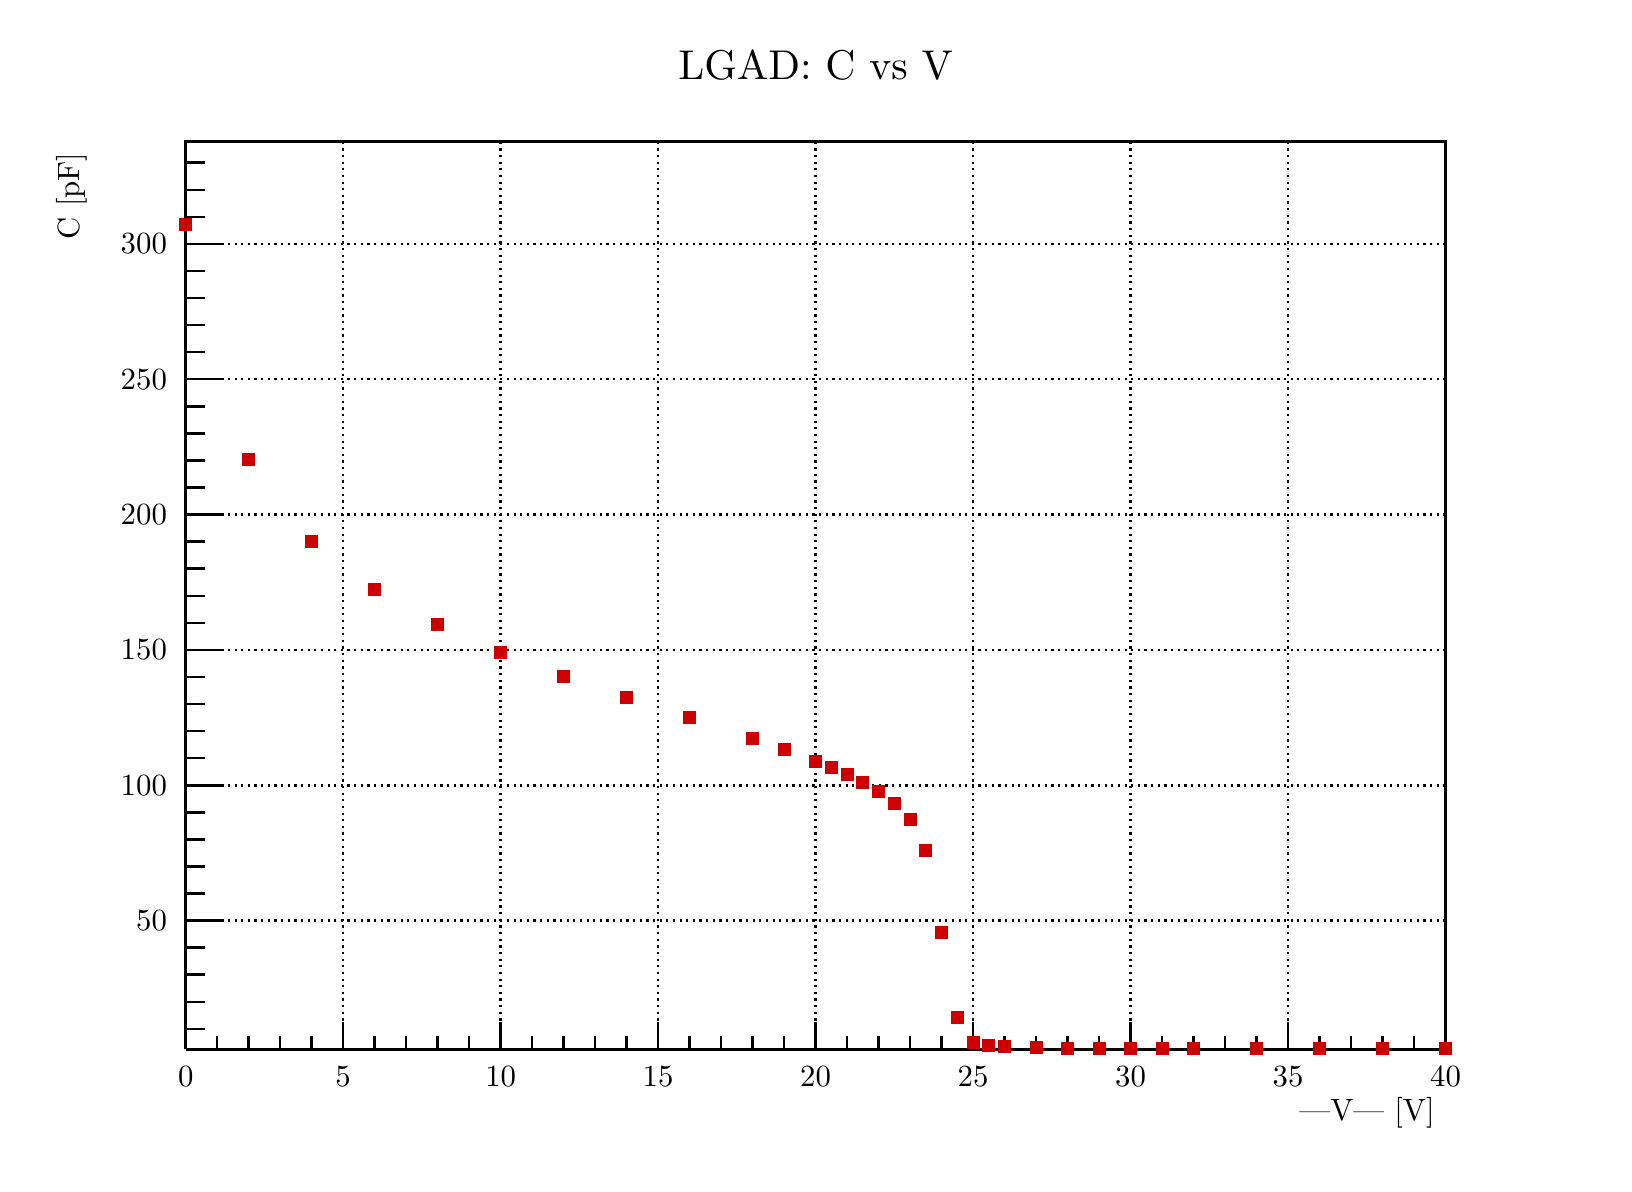
\begin{tikzpicture}
\def\CheckTikzLibraryLoaded#1{ \ifcsname tikz@library@#1@loaded\endcsname \else \PackageWarning{tikz}{usetikzlibrary{#1} is missing in the preamble.} \fi }
\CheckTikzLibraryLoaded{patterns}
\CheckTikzLibraryLoaded{plotmarks}
\pgfdeclareplotmark{cross} {
\pgfpathmoveto{\pgfpoint{-0.3\pgfplotmarksize}{\pgfplotmarksize}}
\pgfpathlineto{\pgfpoint{+0.3\pgfplotmarksize}{\pgfplotmarksize}}
\pgfpathlineto{\pgfpoint{+0.3\pgfplotmarksize}{0.3\pgfplotmarksize}}
\pgfpathlineto{\pgfpoint{+1\pgfplotmarksize}{0.3\pgfplotmarksize}}
\pgfpathlineto{\pgfpoint{+1\pgfplotmarksize}{-0.3\pgfplotmarksize}}
\pgfpathlineto{\pgfpoint{+0.3\pgfplotmarksize}{-0.3\pgfplotmarksize}}
\pgfpathlineto{\pgfpoint{+0.3\pgfplotmarksize}{-1.\pgfplotmarksize}}
\pgfpathlineto{\pgfpoint{-0.3\pgfplotmarksize}{-1.\pgfplotmarksize}}
\pgfpathlineto{\pgfpoint{-0.3\pgfplotmarksize}{-0.3\pgfplotmarksize}}
\pgfpathlineto{\pgfpoint{-1.\pgfplotmarksize}{-0.3\pgfplotmarksize}}
\pgfpathlineto{\pgfpoint{-1.\pgfplotmarksize}{0.3\pgfplotmarksize}}
\pgfpathlineto{\pgfpoint{-0.3\pgfplotmarksize}{0.3\pgfplotmarksize}}
\pgfpathclose
\pgfusepathqstroke
}
\pgfdeclareplotmark{cross*} {
\pgfpathmoveto{\pgfpoint{-0.3\pgfplotmarksize}{\pgfplotmarksize}}
\pgfpathlineto{\pgfpoint{+0.3\pgfplotmarksize}{\pgfplotmarksize}}
\pgfpathlineto{\pgfpoint{+0.3\pgfplotmarksize}{0.3\pgfplotmarksize}}
\pgfpathlineto{\pgfpoint{+1\pgfplotmarksize}{0.3\pgfplotmarksize}}
\pgfpathlineto{\pgfpoint{+1\pgfplotmarksize}{-0.3\pgfplotmarksize}}
\pgfpathlineto{\pgfpoint{+0.3\pgfplotmarksize}{-0.3\pgfplotmarksize}}
\pgfpathlineto{\pgfpoint{+0.3\pgfplotmarksize}{-1.\pgfplotmarksize}}
\pgfpathlineto{\pgfpoint{-0.3\pgfplotmarksize}{-1.\pgfplotmarksize}}
\pgfpathlineto{\pgfpoint{-0.3\pgfplotmarksize}{-0.3\pgfplotmarksize}}
\pgfpathlineto{\pgfpoint{-1.\pgfplotmarksize}{-0.3\pgfplotmarksize}}
\pgfpathlineto{\pgfpoint{-1.\pgfplotmarksize}{0.3\pgfplotmarksize}}
\pgfpathlineto{\pgfpoint{-0.3\pgfplotmarksize}{0.3\pgfplotmarksize}}
\pgfpathclose
\pgfusepathqfillstroke
}
\pgfdeclareplotmark{newstar} {
\pgfpathmoveto{\pgfqpoint{0pt}{\pgfplotmarksize}}
\pgfpathlineto{\pgfqpointpolar{44}{0.5\pgfplotmarksize}}
\pgfpathlineto{\pgfqpointpolar{18}{\pgfplotmarksize}}
\pgfpathlineto{\pgfqpointpolar{-20}{0.5\pgfplotmarksize}}
\pgfpathlineto{\pgfqpointpolar{-54}{\pgfplotmarksize}}
\pgfpathlineto{\pgfqpointpolar{-90}{0.5\pgfplotmarksize}}
\pgfpathlineto{\pgfqpointpolar{234}{\pgfplotmarksize}}
\pgfpathlineto{\pgfqpointpolar{198}{0.5\pgfplotmarksize}}
\pgfpathlineto{\pgfqpointpolar{162}{\pgfplotmarksize}}
\pgfpathlineto{\pgfqpointpolar{134}{0.5\pgfplotmarksize}}
\pgfpathclose
\pgfusepathqstroke
}
\pgfdeclareplotmark{newstar*} {
\pgfpathmoveto{\pgfqpoint{0pt}{\pgfplotmarksize}}
\pgfpathlineto{\pgfqpointpolar{44}{0.5\pgfplotmarksize}}
\pgfpathlineto{\pgfqpointpolar{18}{\pgfplotmarksize}}
\pgfpathlineto{\pgfqpointpolar{-20}{0.5\pgfplotmarksize}}
\pgfpathlineto{\pgfqpointpolar{-54}{\pgfplotmarksize}}
\pgfpathlineto{\pgfqpointpolar{-90}{0.5\pgfplotmarksize}}
\pgfpathlineto{\pgfqpointpolar{234}{\pgfplotmarksize}}
\pgfpathlineto{\pgfqpointpolar{198}{0.5\pgfplotmarksize}}
\pgfpathlineto{\pgfqpointpolar{162}{\pgfplotmarksize}}
\pgfpathlineto{\pgfqpointpolar{134}{0.5\pgfplotmarksize}}
\pgfpathclose
\pgfusepathqfillstroke
}
\definecolor{c}{rgb}{1,1,1};
\draw [color=c, fill=c] (0,0) rectangle (20,14.411);
\draw [color=c, fill=c] (2,1.4411) rectangle (18,12.9699);
\definecolor{c}{rgb}{0,0,0};
\draw [c,line width=0.9] (2,1.4411) -- (2,12.9699) -- (18,12.9699) -- (18,1.4411) -- (2,1.4411);
\definecolor{c}{rgb}{1,1,1};
\draw [color=c, fill=c] (2,1.4411) rectangle (18,12.9699);
\definecolor{c}{rgb}{0,0,0};
\draw [c,line width=0.9] (2,1.4411) -- (2,12.9699) -- (18,12.9699) -- (18,1.4411) -- (2,1.4411);
\draw [c,line width=0.9] (2,1.4411) -- (18,1.4411);
\draw [c,dash pattern=on 0.80pt off 1.60pt ,line width=0.9] (2,12.9699) -- (2,1.4411);
\draw [c,dash pattern=on 0.80pt off 1.60pt ,line width=0.9] (4,12.9699) -- (4,1.4411);
\draw [c,dash pattern=on 0.80pt off 1.60pt ,line width=0.9] (6,12.9699) -- (6,1.4411);
\draw [c,dash pattern=on 0.80pt off 1.60pt ,line width=0.9] (8,12.9699) -- (8,1.4411);
\draw [c,dash pattern=on 0.80pt off 1.60pt ,line width=0.9] (10,12.9699) -- (10,1.4411);
\draw [c,dash pattern=on 0.80pt off 1.60pt ,line width=0.9] (12,12.9699) -- (12,1.4411);
\draw [c,dash pattern=on 0.80pt off 1.60pt ,line width=0.9] (14,12.9699) -- (14,1.4411);
\draw [c,dash pattern=on 0.80pt off 1.60pt ,line width=0.9] (16,12.9699) -- (16,1.4411);
\draw [c,dash pattern=on 0.80pt off 1.60pt ,line width=0.9] (18,12.9699) -- (18,1.4411);
\draw [c,line width=0.9] (2,1.4411) -- (2,12.9699);
\draw [c,dash pattern=on 0.80pt off 1.60pt ,line width=0.9] (18,3.07789) -- (2,3.07789);
\draw [c,dash pattern=on 0.80pt off 1.60pt ,line width=0.9] (18,4.79666) -- (2,4.79666);
\draw [c,dash pattern=on 0.80pt off 1.60pt ,line width=0.9] (18,6.51543) -- (2,6.51543);
\draw [c,dash pattern=on 0.80pt off 1.60pt ,line width=0.9] (18,8.2342) -- (2,8.2342);
\draw [c,dash pattern=on 0.80pt off 1.60pt ,line width=0.9] (18,9.95297) -- (2,9.95297);
\draw [c,dash pattern=on 0.80pt off 1.60pt ,line width=0.9] (18,11.6717) -- (2,11.6717);
\draw [c,dash pattern=on 0.80pt off 1.60pt ,line width=0.9] (18,3.07789) -- (2,3.07789);
\draw [c,dash pattern=on 0.80pt off 1.60pt ,line width=0.9] (18,11.6717) -- (2,11.6717);
\draw [c,line width=0.9] (2,1.4411) -- (18,1.4411);
\draw [c,line width=0.9] (2,1.78697) -- (2,1.4411);
\draw [c,line width=0.9] (2.4,1.61404) -- (2.4,1.4411);
\draw [c,line width=0.9] (2.8,1.61404) -- (2.8,1.4411);
\draw [c,line width=0.9] (3.2,1.61404) -- (3.2,1.4411);
\draw [c,line width=0.9] (3.6,1.61404) -- (3.6,1.4411);
\draw [c,line width=0.9] (4,1.78697) -- (4,1.4411);
\draw [c,line width=0.9] (4.4,1.61404) -- (4.4,1.4411);
\draw [c,line width=0.9] (4.8,1.61404) -- (4.8,1.4411);
\draw [c,line width=0.9] (5.2,1.61404) -- (5.2,1.4411);
\draw [c,line width=0.9] (5.6,1.61404) -- (5.6,1.4411);
\draw [c,line width=0.9] (6,1.78697) -- (6,1.4411);
\draw [c,line width=0.9] (6.4,1.61404) -- (6.4,1.4411);
\draw [c,line width=0.9] (6.8,1.61404) -- (6.8,1.4411);
\draw [c,line width=0.9] (7.2,1.61404) -- (7.2,1.4411);
\draw [c,line width=0.9] (7.6,1.61404) -- (7.6,1.4411);
\draw [c,line width=0.9] (8,1.78697) -- (8,1.4411);
\draw [c,line width=0.9] (8.4,1.61404) -- (8.4,1.4411);
\draw [c,line width=0.9] (8.8,1.61404) -- (8.8,1.4411);
\draw [c,line width=0.9] (9.2,1.61404) -- (9.2,1.4411);
\draw [c,line width=0.9] (9.6,1.61404) -- (9.6,1.4411);
\draw [c,line width=0.9] (10,1.78697) -- (10,1.4411);
\draw [c,line width=0.9] (10.4,1.61404) -- (10.4,1.4411);
\draw [c,line width=0.9] (10.8,1.61404) -- (10.8,1.4411);
\draw [c,line width=0.9] (11.2,1.61404) -- (11.2,1.4411);
\draw [c,line width=0.9] (11.6,1.61404) -- (11.6,1.4411);
\draw [c,line width=0.9] (12,1.78697) -- (12,1.4411);
\draw [c,line width=0.9] (12.4,1.61404) -- (12.4,1.4411);
\draw [c,line width=0.9] (12.8,1.61404) -- (12.8,1.4411);
\draw [c,line width=0.9] (13.2,1.61404) -- (13.2,1.4411);
\draw [c,line width=0.9] (13.6,1.61404) -- (13.6,1.4411);
\draw [c,line width=0.9] (14,1.78697) -- (14,1.4411);
\draw [c,line width=0.9] (14.4,1.61404) -- (14.4,1.4411);
\draw [c,line width=0.9] (14.8,1.61404) -- (14.8,1.4411);
\draw [c,line width=0.9] (15.2,1.61404) -- (15.2,1.4411);
\draw [c,line width=0.9] (15.6,1.61404) -- (15.6,1.4411);
\draw [c,line width=0.9] (16,1.78697) -- (16,1.4411);
\draw [c,line width=0.9] (16.4,1.61404) -- (16.4,1.4411);
\draw [c,line width=0.9] (16.8,1.61404) -- (16.8,1.4411);
\draw [c,line width=0.9] (17.2,1.61404) -- (17.2,1.4411);
\draw [c,line width=0.9] (17.6,1.61404) -- (17.6,1.4411);
\draw [c,line width=0.9] (18,1.78697) -- (18,1.4411);
\draw [anchor=base] (2,0.965539) node[scale=1.11327, color=c, rotate=0]{0};
\draw [anchor=base] (4,0.965539) node[scale=1.11327, color=c, rotate=0]{5};
\draw [anchor=base] (6,0.965539) node[scale=1.11327, color=c, rotate=0]{10};
\draw [anchor=base] (8,0.965539) node[scale=1.11327, color=c, rotate=0]{15};
\draw [anchor=base] (10,0.965539) node[scale=1.11327, color=c, rotate=0]{20};
\draw [anchor=base] (12,0.965539) node[scale=1.11327, color=c, rotate=0]{25};
\draw [anchor=base] (14,0.965539) node[scale=1.11327, color=c, rotate=0]{30};
\draw [anchor=base] (16,0.965539) node[scale=1.11327, color=c, rotate=0]{35};
\draw [anchor=base] (18,0.965539) node[scale=1.11327, color=c, rotate=0]{40};
\draw [anchor= east] (18,0.634085) node[scale=1.11327, color=c, rotate=0]{|V| [V]};
\draw [c,line width=0.9] (2,1.4411) -- (2,12.9699);
\draw [c,line width=0.9] (2.48,3.07789) -- (2,3.07789);
\draw [c,line width=0.9] (2.24,3.42164) -- (2,3.42164);
\draw [c,line width=0.9] (2.24,3.7654) -- (2,3.7654);
\draw [c,line width=0.9] (2.24,4.10915) -- (2,4.10915);
\draw [c,line width=0.9] (2.24,4.4529) -- (2,4.4529);
\draw [c,line width=0.9] (2.48,4.79666) -- (2,4.79666);
\draw [c,line width=0.9] (2.24,5.14041) -- (2,5.14041);
\draw [c,line width=0.9] (2.24,5.48417) -- (2,5.48417);
\draw [c,line width=0.9] (2.24,5.82792) -- (2,5.82792);
\draw [c,line width=0.9] (2.24,6.17167) -- (2,6.17167);
\draw [c,line width=0.9] (2.48,6.51543) -- (2,6.51543);
\draw [c,line width=0.9] (2.24,6.85918) -- (2,6.85918);
\draw [c,line width=0.9] (2.24,7.20294) -- (2,7.20294);
\draw [c,line width=0.9] (2.24,7.54669) -- (2,7.54669);
\draw [c,line width=0.9] (2.24,7.89044) -- (2,7.89044);
\draw [c,line width=0.9] (2.48,8.2342) -- (2,8.2342);
\draw [c,line width=0.9] (2.24,8.57795) -- (2,8.57795);
\draw [c,line width=0.9] (2.24,8.92171) -- (2,8.92171);
\draw [c,line width=0.9] (2.24,9.26546) -- (2,9.26546);
\draw [c,line width=0.9] (2.24,9.60921) -- (2,9.60921);
\draw [c,line width=0.9] (2.48,9.95297) -- (2,9.95297);
\draw [c,line width=0.9] (2.24,10.2967) -- (2,10.2967);
\draw [c,line width=0.9] (2.24,10.6405) -- (2,10.6405);
\draw [c,line width=0.9] (2.24,10.9842) -- (2,10.9842);
\draw [c,line width=0.9] (2.24,11.328) -- (2,11.328);
\draw [c,line width=0.9] (2.48,11.6717) -- (2,11.6717);
\draw [c,line width=0.9] (2.48,3.07789) -- (2,3.07789);
\draw [c,line width=0.9] (2.24,2.73413) -- (2,2.73413);
\draw [c,line width=0.9] (2.24,2.39038) -- (2,2.39038);
\draw [c,line width=0.9] (2.24,2.04663) -- (2,2.04663);
\draw [c,line width=0.9] (2.24,1.70287) -- (2,1.70287);
\draw [c,line width=0.9] (2.48,11.6717) -- (2,11.6717);
\draw [c,line width=0.9] (2.24,12.0155) -- (2,12.0155);
\draw [c,line width=0.9] (2.24,12.3592) -- (2,12.3592);
\draw [c,line width=0.9] (2.24,12.703) -- (2,12.703);
\draw [anchor= east] (1.9,3.07789) node[scale=1.11327, color=c, rotate=0]{50};
\draw [anchor= east] (1.9,4.79666) node[scale=1.11327, color=c, rotate=0]{100};
\draw [anchor= east] (1.9,6.51543) node[scale=1.11327, color=c, rotate=0]{150};
\draw [anchor= east] (1.9,8.2342) node[scale=1.11327, color=c, rotate=0]{200};
\draw [anchor= east] (1.9,9.95297) node[scale=1.11327, color=c, rotate=0]{250};
\draw [anchor= east] (1.9,11.6717) node[scale=1.11327, color=c, rotate=0]{300};
\draw [anchor= east] (0.54812,12.9699) node[scale=1.11327, color=c, rotate=90]{C [pF]};
\definecolor{c}{rgb}{0.8,0,0};
\foreach \P in {(2,11.9192), (2.8,8.93374), (3.6,7.89423), (4.4,7.27925), (5.2,6.83684), (6,6.48105), (6.8,6.18164), (7.6,5.91076), (8.4,5.65364), (9.2,5.39341), (9.6,5.25591), (10,5.10294), (10.2,5.02044), (10.4,4.93038), (10.6,4.83),
 (10.8,4.71278), (11,4.56703), (11.2,4.36009), (11.4,3.9689), (11.6,2.9232), (11.8,1.84622), (12,1.52446), (12.2,1.49043), (12.4,1.47324), (12.8,1.4619), (13.2,1.45674), (13.6,1.45502), (14,1.45399), (14.4,1.45331), (14.8,1.45193), (15.6,1.45262),
 (16.4,1.45262), (17.2,1.45227), (18,1.45193)}{\draw[mark options={color=c,fill=c},mark size=2.162162pt, line width=0.000000pt, mark=square*] plot coordinates {\P};}
\definecolor{c}{rgb}{0,0,0};
\draw (10,13.9427) node[scale=1.50291, color=c, rotate=0]{LGAD: C vs V};
\end{tikzpicture}
%\end{document}
